\section{Receiver Observables and Signal Tracking}
\label{sec:signal}

The detectors evaluated here operate on observables a receiver computes while tracking a
signal. This section specifies the processing that produces them, the observable set
retained, the criterion by which that set was selected, and the labelling procedure, so
that the effect of a transmitted attack on each quantity can be traced through the chain.

\subsection{Receiver processing}

A GPS L1 C/A satellite transmits a carrier modulated by a pseudorandom spreading code of
1023 chips repeating every millisecond, and by navigation data at 50 bits per second. The
code is public and distinct for each satellite, which is what permits a counterfeit to be
generated at all.

Reception proceeds in two stages. In acquisition the receiver searches jointly over code
phase and carrier frequency until it finds the alignment at which its locally generated
replica correlates strongly with the incoming signal. In tracking it maintains that
alignment as the satellite geometry and the receiver clock evolve. Tracking is implemented
by three feedback loops operating concurrently. The delay locked loop maintains code
alignment by correlating the incoming signal against early, prompt and late replicas and
steering so that the early and late correlations remain equal, which holds the prompt
replica on the correlation peak. The phase locked loop maintains carrier phase alignment.
The frequency locked loop performs the equivalent function for carrier frequency and is
more tolerant of low signal to noise ratio, so it assists when phase lock is marginal.

The loops produce a set of quantities at each integration interval. These quantities are
the detector inputs used throughout this study. They are not selected for convenience of
classification: they are what the receiver computes in order to function, and a detector
operating inside a receiver would have access to precisely this set.

\subsection{Observable measurements}
\label{sec:features}

Table~\ref{tab:features} lists the nine measurements, exported once per epoch for each
tracked satellite.

\begin{table}[t]
\centering
\caption{The nine measurements each detector reads, per satellite per epoch.}
\label{tab:features}
\begin{tabular}{@{}llp{5.1cm}@{}}
\toprule
Measurement & Units & What it is \\
\midrule
$C/N_0$              & dB-Hz  & Received signal strength relative to the noise density \\
Mean $C/N_0$         & dB-Hz  & The same, averaged over the preceding second \\
Noise estimate       & --     & Correlator output away from the peak, used as the noise
                                reference \\
Doppler              & Hz     & Frequency offset of the carrier from its nominal value \\
Prompt in phase      & --     & Correlation with the on peak code copy, in phase
                                component \\
Prompt quadrature    & --     & The same, quadrature component \\
Delay lock discriminator & chips & Difference between the early and late correlations,
                                the code tracking error \\
Phase lock indicator & --     & How well the phase locked loop is holding \\
Frequency lock indicator & -- & How well the frequency locked loop is holding \\
\bottomrule
\end{tabular}
\end{table}

The set spans the three aspects of tracking that a spoofing attack perturbs. Received
power is represented by the first three entries, which respond to the counterfeit's
transmitted power relative to the authentic signal. Carrier behaviour is represented by
the Doppler, the two prompt correlator components and the phase and frequency lock
indicators, which respond to the counterfeit's carrier frequency and phase. Code behaviour
is represented by the delay lock discriminator, which responds to the displacement between
the counterfeit code and the authentic code and therefore to the pull-off rate.
Figure~\ref{fig:featdist} shows the marginal distribution of each observable under the two
classes; the classes overlap in every single observable, which is why a learned detector
that combines them can outperform any univariate threshold.

% Figure source: figures_src/fig_legacy.py
\begin{figure*}[t]
\centering
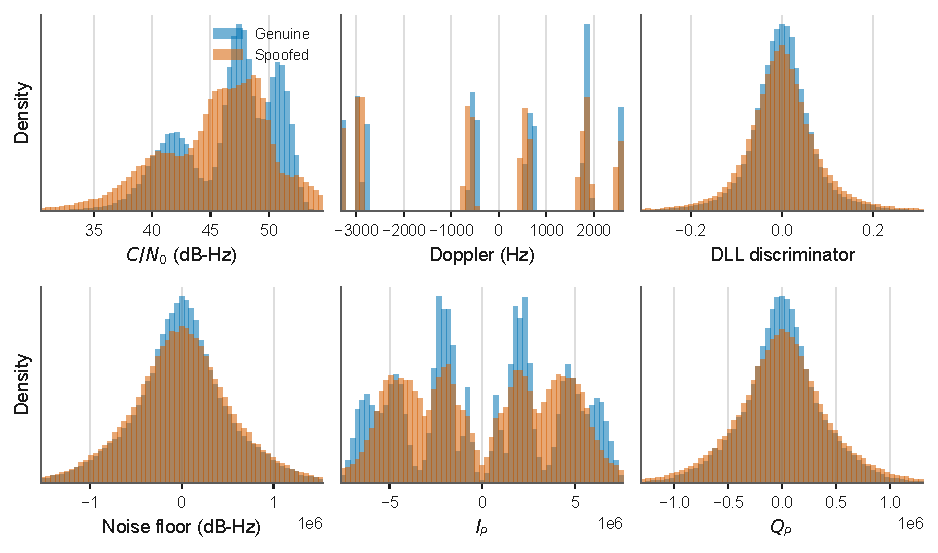
\includegraphics[width=\textwidth]{figures/fig03_feature_distributions.pdf}
\caption{Distribution of each of the nine measurements for authentic and for spoofed epochs. The classes overlap in every measurement, which is why a detector combines them instead of thresholding any one.}
\label{fig:featdist}
\end{figure*}

\subsection{Selection of the observable set}

A software receiver exposes more quantities than the nine retained, and several of the
additional ones are exact deterministic functions of quantities already in the set. The
prompt correlator power is the sum of squares of the two prompt components; the prompt
phase is the arctangent of their ratio; the carrier frequency is the Doppler displaced by
a fixed nominal value.

Such derived quantities are excluded, for two reasons. They contribute no information
beyond their parents, so their inclusion cannot improve an optimal classifier. More
importantly, their presence would admit an evaluation artefact: a perturbation that
displaced a derived quantity without correspondingly displacing its parents specifies a
receiver state that no incident waveform can produce, and any attack exploiting such a
displacement would be an artefact of the feature representation. The nine retained
observables are functionally independent, in the sense that none is an exact function of
the others, which eliminates that particular failure mode.

Functional independence is a property of the representation and does not by itself
establish that an arbitrary configuration of the nine is physically attainable, since
independence among coordinates says nothing about the image of the map from transmitter
parameters to observables. In the waveform level evaluation the question is not reached,
because the observables are by construction whatever the receiver computes while tracking
a transmitted signal. It is reached in the feature space comparison of
Section~\ref{sec:res_compare}, and is treated there.
Figure~\ref{fig:timehistory} shows the joint evolution of the observables for one satellite
across the onset of a recorded attack.

% Figure source: figures_src/fig_legacy.py
\begin{figure*}[t]
\centering
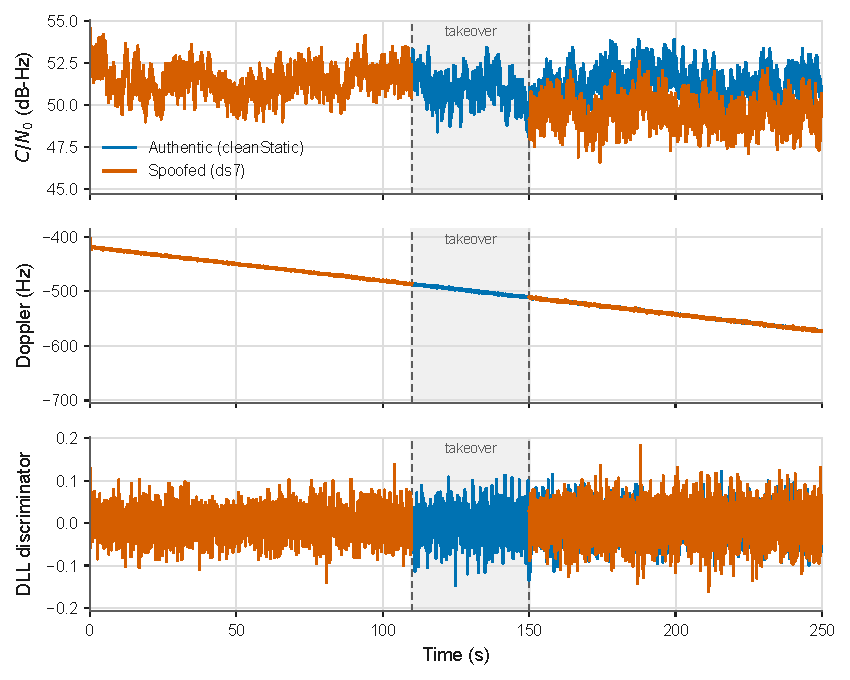
\includegraphics[width=\textwidth]{figures/fig02_signature_timehistory_prn23.pdf}
\caption{Time history of the measurements for one satellite, pseudorandom noise (PRN) code 23, across the onset of a recorded attack. The measurements move together as the counterfeit takes over the tracking loops, which is the signature a detector reads.}
\label{fig:timehistory}
\end{figure*}

\subsection{Labelling and data partitioning}

Each epoch is labelled according to whether the signal being tracked at that instant was
authentic or contained a counterfeit, following the documented onset time within each
recording. Epochs spanning the takeover transient are discarded, because during handover
the tracked signal is neither fully authentic nor fully under the adversary's control and
the label would be ambiguous.

Both classes are drawn from within the same recording. This is a deliberate constraint on
corpus construction. Were authentic epochs taken from one recording and spoofed epochs
from another, a classifier could attain high apparent accuracy by identifying the
recording of origin through front end, antenna or clock characteristics, which is not
spoofing detection and would not transfer to deployment. Drawing both classes from a
single recording, with a common front end and a common clock, removes that confound.

Training, validation and test partitions are taken as disjoint contiguous blocks in time,
with a margin discarded at each boundary. Adjacent epochs of the same satellite are
strongly correlated, since the observables evolve continuously and the integration
interval is short relative to the dynamics, so a randomised partition would place near
duplicates of the same observation on both sides of the split and inflate the measured
accuracy.
